\documentclass{article}
\usepackage{arxiv}
\usepackage[utf8]{inputenc} % allow utf-8 input
\usepackage[T1]{fontenc}    % use 8-bit T1 fonts
\usepackage{hyperref}       % hyperlinks
\usepackage{url}            % simple URL typesetting
\usepackage{booktabs}       % professional-quality tables
\usepackage{amsfonts}       % blackboard math symbols
\usepackage{nicefrac}       % compact symbols for 1/2, etc.
\usepackage{microtype}      % microtypography
\usepackage{lipsum}		% Can be removed after putting your text content
\usepackage{graphicx}
\usepackage{natbib}
\usepackage{doi}

\title{Survey of Self-Supervised Learning approaches in Graph Machine Learning}

\author{ \href{https://kushajveersingh.github.io}{Kushajveer Singh} \\
	University of Georgia\\
	\texttt{Kushajveer.Singh@uga.edu}
}

\hypersetup{
pdftitle={Survey of Self-Supervised Learning approaches in Graph Machine Learning},
pdfauthor={Kushajveer Singh},
pdfkeywords={Self-supervised learning, graph neural networks, deep learning, unsupervised learning, graph analysis, survey, review},
}

\begin{document}
\maketitle

\begin{abstract}
	Deep learning has achieved remarkable success on a variety of tasks, especially in recent years where a new field of deep learning, called Graph Machine Learning (GML), has achieved tremendous success with non-euclidean data (graphs). Self-supervised learning (SSL) is emerging as a new paradigm for making use of large amounts of unlabeled samples. SSL has achieved promising results in the field of computer vision and natural language processing and is slowing making its way to GML as well. Graph Neural Networks (GNNs) serve as the backbone of these SSL methods and in this survey, we provide a review of different ways SSL is being employed in GML. Specifically, we categorize SSL methods in contrastive and predictive models and then discuss various techniques used in each category. We also discuss the datasets used to test various SSL approaches and the evaluation metrics to compare these methods. We also provide an implementation of a GNN model that achieves strong results on ogbn-arxiv dataset and can be used as a backbone for the methods discussed in paper.
\end{abstract}


% keywords can be removed
\keywords{Self-supervised learning, graph neural networks, deep learning, unsupervised learning, graph analysis, survey, review}

\section{Introduction}
In Deep Learning, we create a model that takes some data as input and is trained to output desired predictions. This is called supervised learning and it has been leading the success of Deep Learning for years since AlexNet \citep{alexnet}. The biggest problem is collection of labels and a followup problem is how to make use of a large amount of unlabeled data that is available for free. This new paradigm is called self-supervised learning which collectively refers to unsupervised representation learning, unsupervised pretraining and auxiliary training.

A common way to train a deep model is to use supervised learning in which a sufficient amount of input data and label pairs are given. However, since a large amount of labeled data is required supervised learning becomes expensive. In such cases, self-supervised learning (SSL) enables the training of deep models on unlabeled data, removing the need of labels by generating labels itself. When a limited amount of data is available, SSL can be used to pretrain the model on unlabeled data and then finetuned on the downstream task with supervised learning \citep{finetune1, finetune2}.

Recently SSL has shown remarkable success in image super-resolution \citep{example1}, image denoising \citep{example2, example3}, visual representation \citep{example4, example5, example6}, language sequences \citep{example7, example8}. SSL has also been applied to graphs with sequence models \citep{example9, example10}. Taking the image domain as an example, SimCLR \citep{example11} proposed a novel constrastive loss where we find positive and negative views of an image and compute a normalized softmax over different views in a batch, MoCo \citep{example12} propose an unsupervised visual representation learning framework for learning on-the-fly contrastive representations of an image, \citep{example13, example14} design different pretext tasks to train convolutional neural networks (CNNs) to capture relationships between different crops from an image.

SSL methods work by creating pseudo labels/data to create the training signal. The labels are generated by pretext tasks, these tasks are general tasks that can generate their own labels. For example, dividing an image into a 3x3 grid and identifying which square goes at a particular location. Based on how the pretext task is defined SSL methods can be divided into two categories; namely contrastive models and predictive models. The major difference between these two approaches is in contrastive models, we generate data-data pairs and then pass these pairs into a contrastive loss, while in predictive models we generate data-label pairs and use a supervised style loss to train the model. Figure \ref{fig:fig1} shows a comparison between the contrastive and predictive model discussed in this section.

\begin{figure}
	\centering
	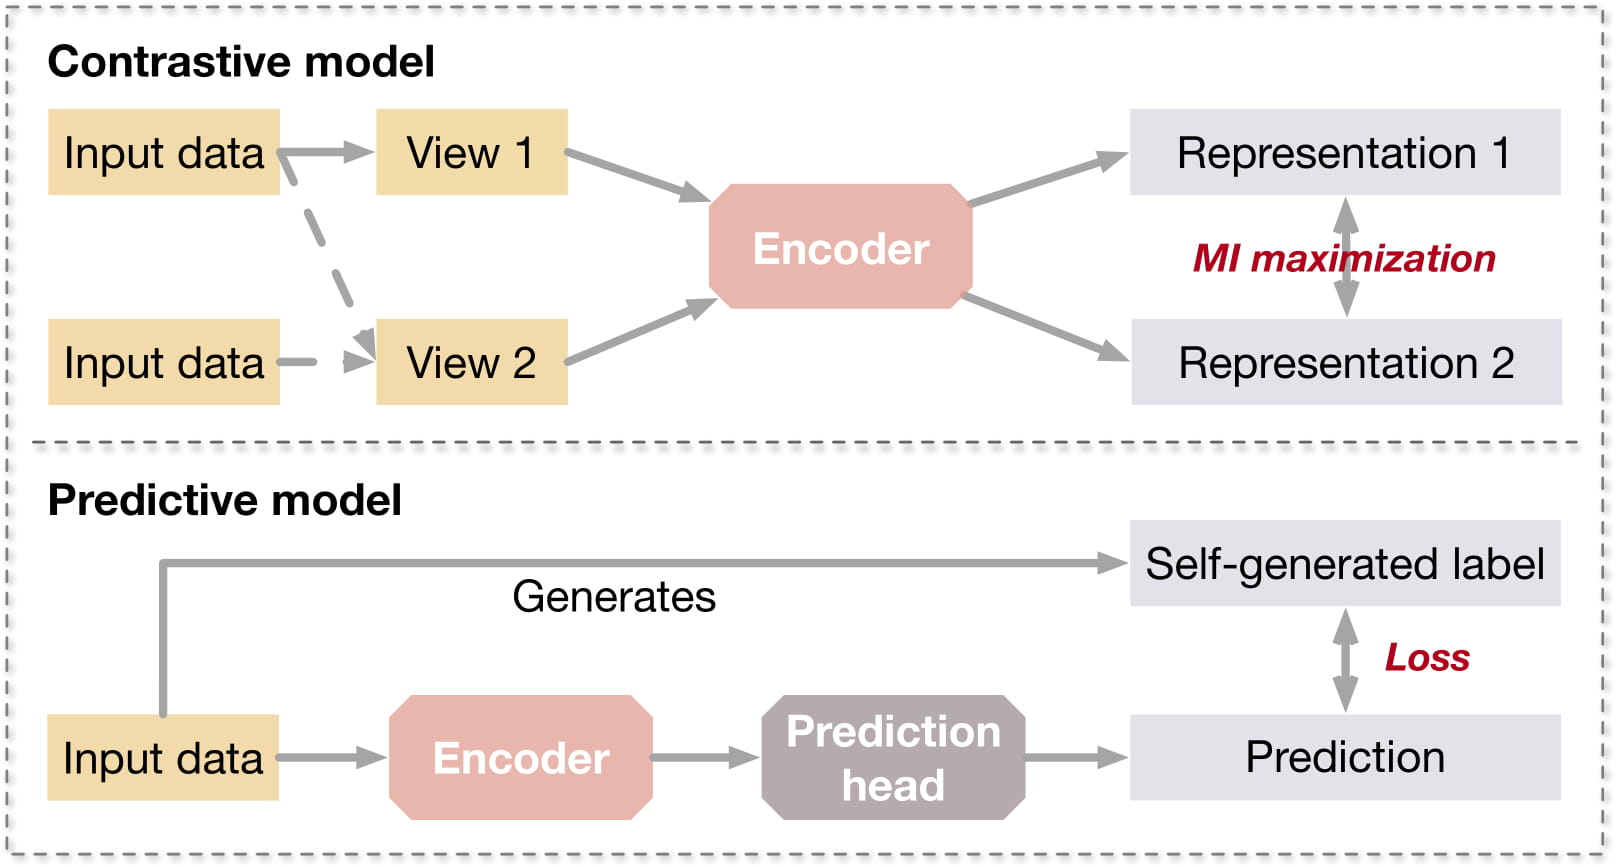
\includegraphics[scale=0.2]{figure1.jpg}
	\caption{A comparison between the contrastive model and the predictive model in general. Figure taken from \citep{cite1}}
	\label{fig:fig1}
\end{figure}

Contrastive methods work by minimizing a energy function. The energy function is pushed down at every positive data-data point and the energy function is pushed up at every negative data-data pair. This is also a limitation of the contrastive methods, because the both the amount of data required and the time required to train the model is very large. In short, contrastive models can be thought to perform discrimination between positive pairs and negative pairs.

Predictive method work in a supervised fashion, where data-label pairs are generated. The labels are generated directly from the input based on certain properties of the input data or selecting certain parts of the data. The architecture for these methods is same as contrastive methods except prediction heads are added on top of the encoder to predict the pseudo labels. When applied to downstream tasks the prediction heads are dropped.

\section{Related work}

In graph data analysis, SSL is very important because graphs occur everywhere and there is massive amount of unlabeled data, such as molecular graphs \citep{cite2, cite3}. To discuss SSL methods, we need to first discuss the graph neural network (GNN) backbones used by these methods. Both contrastive and predictive methods for SSL use a GNN, which we call encoder from now on, as the backbone model. In contrastive methods we pass different views of the graph and use the output of encoder to minimize the energy function. In predictive methods the output of the encoder is used as input to the predictive head which is a MLP in most cases. \citep{cite4} showed that the strength of the encoder is directly proportional to performance of the SSL methods.

GCN \citep{cite5} was the first spectral-based model that was build on top of message passing algorithm \citep{cite6}. Since then a lot of GNN architectures have been introduced. SAGE \citep{cite7} was the first method to apply GNNs on large-scale graphs by sampling a neighborhood of each node, GAT \citep{cite8} added attention weights to the edges, TransformerGNN \citep{cite9} extended transformers from natural language processing to graph based data, by computing the edge using self-attention mechanism. Recently, GCNII \citep{cite10} and GEN \citep{cite11} extended the basic GNN to very deep layers, which was not possible with the previous architectures due to the problem of over-smoothing where the embeddings of all nodes converge to a single point as the depth of the model increases. We use GEN model as the encoder model and reproduce the results of this model on ogbn-arxiv dataset. Details of which are provided in the later sections.

Parallel to this work \citep{cite12} and \cite{cite13} have done an amazing work to summarize the topic as well. Although, the review of these papers is not necessarily up to date with the state of the art, we still borrow some notation from these papers where necessary.

In this paper, we review the latest SSL methods of GNNs and provide a review of both contrastive and predictive methods. We also provide details on how to train a strong encoder model to use as a backbone for these methods. We summarize the contributions of the paper as follows:
\begin{itemize}
    \item We provide an up-to-date review of SSL methods for graph neural networks
    \item We develop a strong encoder model that can be used as a backbone for contrastive and predictive models. To test the performance of the encoder, we compare the accuracy results on ongb-arxiv dataset which is a node-classification dataset.
    \item We provide a summary of various datasets and evaluation metrics that are used to test SSL methods. Previous works only provided information on small scale datasets, but we provide information on large-scale datasets like OGB which are becoming the standard in Graph Machine Learning.
\end{itemize}

\section{Notation}
Consider an undirected graph $G=(V,E)$ where $V$ denotes the set of vertices of length $|V|$ and $E$ denotes the set of edges of length $|E|$. For each vertex we are given a feature vector of dimension $\mathbb{R}^d$, we denote this using $X \in \mathbb{R}^{|V|\times d}$. Now we consider SSL method which can be represented as a function that takes the graph as input and outputs some features for each node i.e. $f: \mathbb{R}^{|V|\times |V|}\times \mathbb{R}^{|V|\times d} \rightarrow \mathbb{R}^{|V|\times q}$. We use $H$ to denote the output of this function i.e. $H = f(E, X)$.

There are three main ways of incorporating self-supervised learning approaches in the training pipeline, these are unsupervised representation learning, unsupervised pretraining, and auxiliary learning.

In \textbf{unsupervised representation learning}, we are only given the graph $G$ i.e. we have access to no features. Most of the problems that fall in this category are related to learning an embedding function which is used to cluster the data like knowledge graphs for missing link prediction.

The \textbf{unsupervised pretraining} is usually performed in two-stage training. We first train the encoder on an arbitrary task, namely contrastive or predictive task and then use the trained encoder as an initialization for the downstream task. An example for this is to pretrain the encoder to do link prediction task and then use the trained encoder to do node classification. The advantage of this process is for the downstream task we require fewer data.

The \textbf{auxiliary learning} also known as joint training is similar to unsupervised pretraining, but it is a one-stage training. In this we add the SSL loss to the downstream task's loss function. So we are jointly optimizing the downstream task and the SSL task. Auxiliary training has been shown to provide better results than unsupervised pretraining in practice.

Next we discuss \textbf{contrastive learning method}. Note that both contrastive and predictive methods are the actual SSL techniques and the three training methods we discussed above are how we want to incorporate the SSL techniques into our training pipeline i.e. do we want to pretrain (\textit{unsupervised pretraining}) using SSL or jointly optimize the training loss and SSL loss (\textit{auxiliary training}) 

\section{Contrastive Learning}
The goal of contrastive learning is to minimize an energy function. This is done by constructing positive and negative data samples and minimizing the energy function at positive data points and maximizing the energy function at negative data points. In practice, given a graph $G$ we construct another view of the graph $G'$ and this $(G, G')$ is termed as a data pair. From this we can construct positive and negative data points.

To construct these positive and negative data points a lot of techniques have been proposed. InforGraph \citep{cite14} contrast on the presence of substructures (like triangles, called cliques), DGI \citep{cite15} relies on maximizing mutual information between path representations and corresponding high-level summaries of graphs, GMI \citep{cite16} directly contrasts node embeddings in different rotations. \citep{cite17, cite18} contrast views between nodes and subgraphs Other methods like MVGRL \citep{cite19}, GCA \citep{cite16} have also been proposed which contrast views between nodes and structurally transformed graphs like modifying the graph by computing the smoothened representation.

\subsection{Objective function}
In the previous section, we discussed how contrastive learning is computing two different views and then using these as positive and negative samples. The next question we try to answer is how to minimize the distance between different views. In short, after we get different views from a graph we compute \textit{mutual information} (MI) between different views. And the idea is MI should be small for views of same graph. Formally mutual information between two views i.e. $h_i$, $h_j$ where $h(\cdot)$ is the output of the encoder is defined as follows
\begin{equation}
    \max_{f} \frac{1}{\sum_{i\neq j} \sigma_{ij}} \left[ \sum_{i \neq j} \sigma_{ij}\textit{I}(h_i, h_j) \right]
\end{equation}

where $\sigma_{ij} \in \{0, 1\}$, and $\sigma_{ij}=1$ if the mutual information is computed between $h_i$ and $h_j$, and $\sigma_{ij}=0$ otherwise. However, in practice it is not possible to compute $\textit{I}$, so we approximate $\textit{I}$ with $\hat{\textit{I}}$. Some of the popular choices for $\hat{\textit{I}}$ are discussed below.

The \textbf{Donsker-Varadhan (DV)} \citep{cite20}, also known as the DV representation of the KL-divergence, is a lower bound to the mutual information and thus can be used to maximize the mutual information. In practice, it is not used much as it is still expensive to compute as compared to the estimations that we discuss next and the results obtained by this are worse than other methods. 

The \textbf{Jensen-Shannon (JS)} estimator is a more efficient estimation and optimization of the mutual information by computing the JS-divergence between $h_i$ and $h_j$.

\textbf{InfoNCE} is another lower bound to mutual information. The intuition behind InfoNCE is that is aims to score the agreement between $h_i$ and $h_j$ higher if the views are from the same instance.

In practice InforNCE has shown to perform better than Jensen-Shannon estimator for a variety of tasks, except molecular tasks where Jensen-Shannon achieves better performance than InfoNCE. One possible explanation for this is in medical data the amount of correlation is high, which makes it difficult to optimize the agreement between different views.

\subsection{Data augmentations}

\begin{figure}
	\centering
	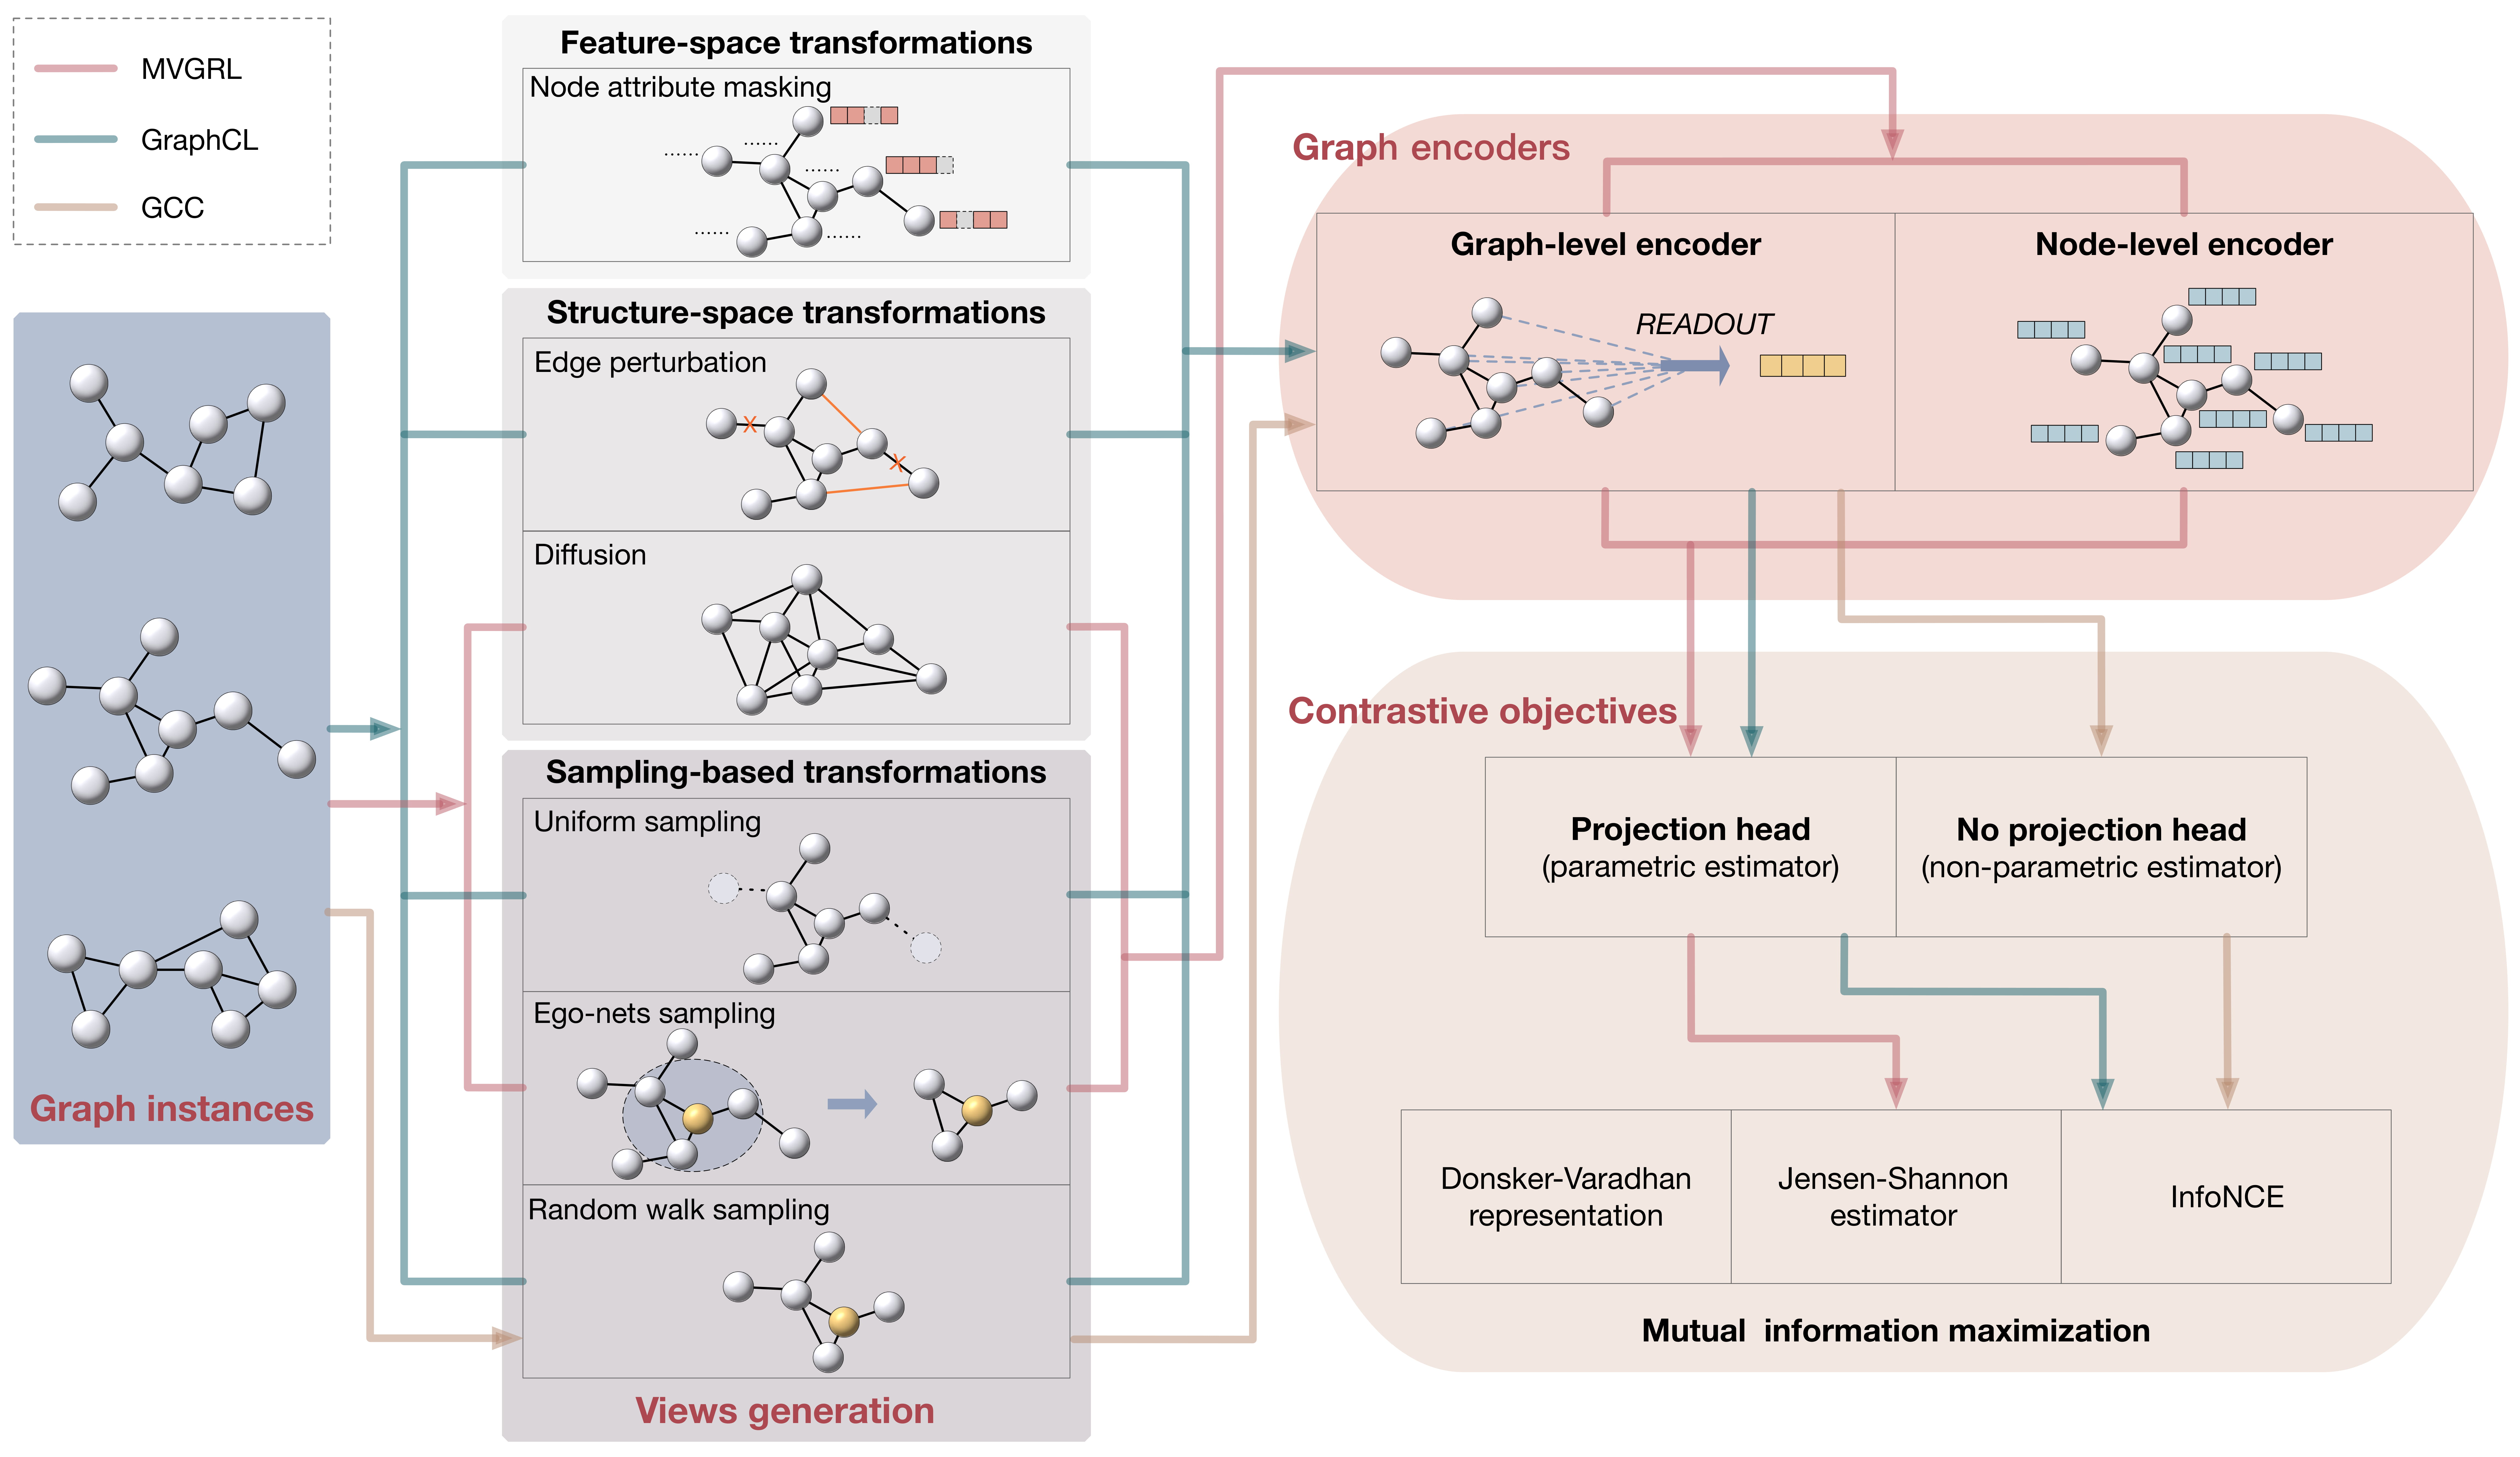
\includegraphics[scale=0.05]{figure2.jpg}
	\caption{Example of various data augmentations used in contrastive methods. Figure taken from \citep{cite1}}
	\label{fig:fig2}
\end{figure}

In this section, we discuss some of the techniques used to generate different views from a graph. These are collectively termed as data augmentations because they allow us to increase the amount of data in the training dataset without having to actually collect more data. Figure \ref{fig:fig2} provides a quick summary of the data augmentations discussed in this section.

\begin{itemize}
    \item \textbf{Node attribute masking}: Mask out some of the input features and replace them with random values. The goal is to predict these missing values. This training pipeline is termed as \textit{denoising autoencoders}.
    \item \textbf{Edge perturbation}: Randomly add or drop some edges in a given graph. This is implemented by adding or dropping values from the adjacency matrix so it is very efficient. The goal is to make the predictions invariant to dropping some random edges.
    \item \textbf{Diffusion}: It is similar edge perturbation, but it uses random walks to add new edges between nodes. In practice, this is implemented by multiplying the adjacency matrix with the diffusion matrix which contains the probability of moving along an edge.
    \item \textbf{Node Dropping}: Randomly remove some nodes based on some pre-computed metrics. For example, nodes can be dropped based on the degree of the nodes and this can improve the fairness metrics of a model.
\end{itemize}

\section{Predictive Learning}
As discussed earlier in predictive learning is similar to supervised learning where pseudo labels are generated and used to provide the supervisory signal for training. These class of methods are much simpler than contrastive methods, as generating labels is a simpler process and less expensive process than computing different views and minimizing the mutual information between the views.

The following methods have shown tremendous success in SLL in recent years
\begin{itemize}
    \item \textbf{GAE} \citep{cite21}: Also known as Variational Autoencoders. These are used to reconstruct the adjacency matrix of a graph. In practice, the task is to predict the existence of an edge between two pairs of nodes and there is no overhead to generate the labels as an adjacency is already available as input.
    \item \textbf{ARGA} \citep{cite22} is an extension of GAE. ARGA is a special case of Variational Autoencoder where we introduce a latent variable in the output distribution to help model all the possible outputs. This makes the learning process a easier to optimize.
\end{itemize}

Predictive methods are generally used in conjunction with contrastive methods, where the autoenocder is used to learn the input distribution for different views.

\section{Evaluation}
A few years back small scale datasets like Cora, Pubmed, Citesser, MoleculeNet were the popular choices for evaluating graph neural networks. But due to the small size of these datasets most of the GNNs saturate and thus it becomes difficult to identify which model performs better than other. Also, it has been shown in recent literature that basic MLPs that take only the node feature information into account can achieve state of the art results which means the edge information is not necessary to get high accuracy on these datasets.

OGB \citep{cite23} is a collection of realistic, large-scale and diverse benchmark datasets for machine learning on graphs. There are three main tasks that we can evaluate the performance of SSL methods using this dataset, namely node classification, link prediction and graph classification. In practice, node classification is used in most of the cases because link prediction is also used as a SSL technique in some approaches and graph classification is same as node classification, with an added global pooling operation.

We used \textbf{ogbn-arxiv} which contains 169,343 nodes 1,166,243 edges as the main dataset. Each node represents an arXiv paper and a paper is connected to another paper if it cite's that paper. The task is to classify each paper/node into 40 categories, where each category represents a tag on arXiv. We trained GEN \citep{cite11} on this dataset and were able to achieve 0.7014 test accuracy without any node classification specific tricks. The code to reproduce the results for this is shared in the zip file and the instructions on how to setup the environment and run the training script are provided in the README.

\subsection{Evaluation metrics}
The goal of SSL is to learn from unlabeled data and as a result generalize when we have small amount of training data available. To reproduce this, most of the SSL methods are evaluated by training on small percentages of the available training data like using 1\%, 5\% of the training data and using the rest as unlabeled data.

\subsection{Conclusion}
Self-supervised learning has recently shown tremendous success in computer vision and natural language processing. Although SSL is still an emerging field when applied to graph data, where some significant challenges need to be addressed. Existing methods apply self-supervision to graph data through either constrastive learning or predictive learning. We presented an introduction to contrastive learning and predictive learning approaches along with a discussion on the recent research applying these methods to graph data. We also provide a summary on what techniques are used in practice along with possible downsides of other methods. To evaluate the SSL methods we discussed why small scale datasets are inappropriate and why the field of graph machine learning is moving to new large-scale benchmark datasets like OGB. Code is also provided which contains the entire training pipeline to train a GNN on one of the OGB datasets.

% \subsection{Tables}
% See awesome Table~\ref{tab:table}.

% The documentation for \verb+booktabs+ (`Publication quality tables in LaTeX') is available from:
% \begin{center}
% 	\url{https://www.ctan.org/pkg/booktabs}
% \end{center}


% \begin{table}
% 	\caption{Sample table title}
% 	\centering
% 	\begin{tabular}{lll}
% 		\toprule
% 		\multicolumn{2}{c}{Part}                   \\
% 		\cmidrule(r){1-2}
% 		Name     & Description     & Size ($\mu$m) \\
% 		\midrule
% 		Dendrite & Input terminal  & $\sim$100     \\
% 		Axon     & Output terminal & $\sim$10      \\
% 		Soma     & Cell body       & up to $10^6$  \\
% 		\bottomrule
% 	\end{tabular}
% 	\label{tab:table}
% \end{table}

\bibliographystyle{unsrtnat}
\bibliography{references}

\end{document}
